\section{Natural Language Processing (NLP)}
The goal of this section is the study of deep neural networks model with a focus on text processing. We will introduce the problem of word representation and solutions to it. To be able to treat those, we will also introduce recurrent neural networks and transformers (this is what is used in general LLM today).

\begin{parag}{Heterogeneous data}
    As we have seen in the section about preprocessing of data. Samples of text can have different size, language etc... For supervised learning task (e.g., sentiment analysis), we assumed the input to always have the same size.
\end{parag}
\begin{parag}{Bag of words}
    Recall on what we have seen before, a way to store data from a text was to actually store the frequency of each word in the text. There BoW encodes an entire document in a single vector, as this is fine for targeted ML task at the document level however this won't work for word-level tasks such as named entity recognition, translation, text generation.
\end{parag}


\begin{parag}{Word representation}
    In neural natural language processing, we treat words as \important{vectors}.
	\begin{center}
	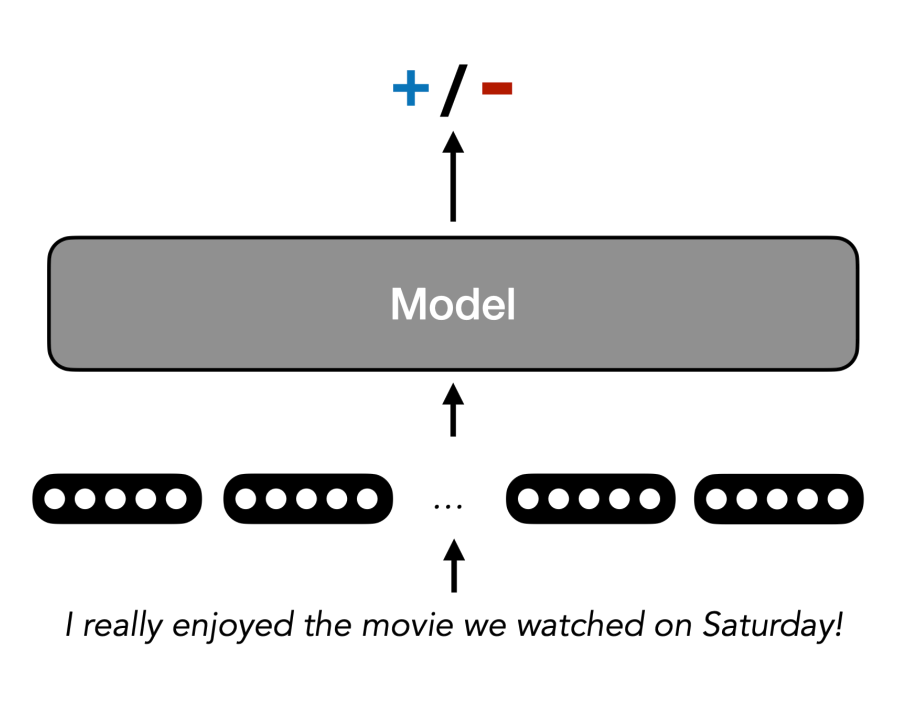
\includegraphics[scale=0.2]{screenshots/2026-05-19.png}
	\end{center}
	A first naive approach to this would be to have a one hot encoding for all words in the vocabulary. We would first define a vocabulary $V$, then we will encode each word into a vector $x_i \in \left\{0, 1\right\}^{\left|V\right|}$. However here we have a big limitation, how do we compute '\textit{similarity}'? We don't have any information if $x$ and $y$ are similar. Let us take for instance the word $house$ and $home$. Those would be pretty similar however in a sparse encoding as defined above this are as similar as $cow$ and $pneumonoultramicroscopicsilicovolcanoconiosis$. We therefore need to have a sort of more complex way of representing our word as a vector. To do so we can introduce word embeddings
\end{parag}

\begin{parag}{Word embeddings}
    Here what we will do is to represent each word as a high-dimensional, real-valued vector (When we say high-dimensional, it is still pretty low in comparison to the $V$ dimension sparse representation but still $O\left(10^2-10^3\right)$). In that case, similarity of vectors represents similarity of meaning for particular words.\\
	$ $\\
	Ultimately the goal would be to have a space as this one below
	\begin{center}
	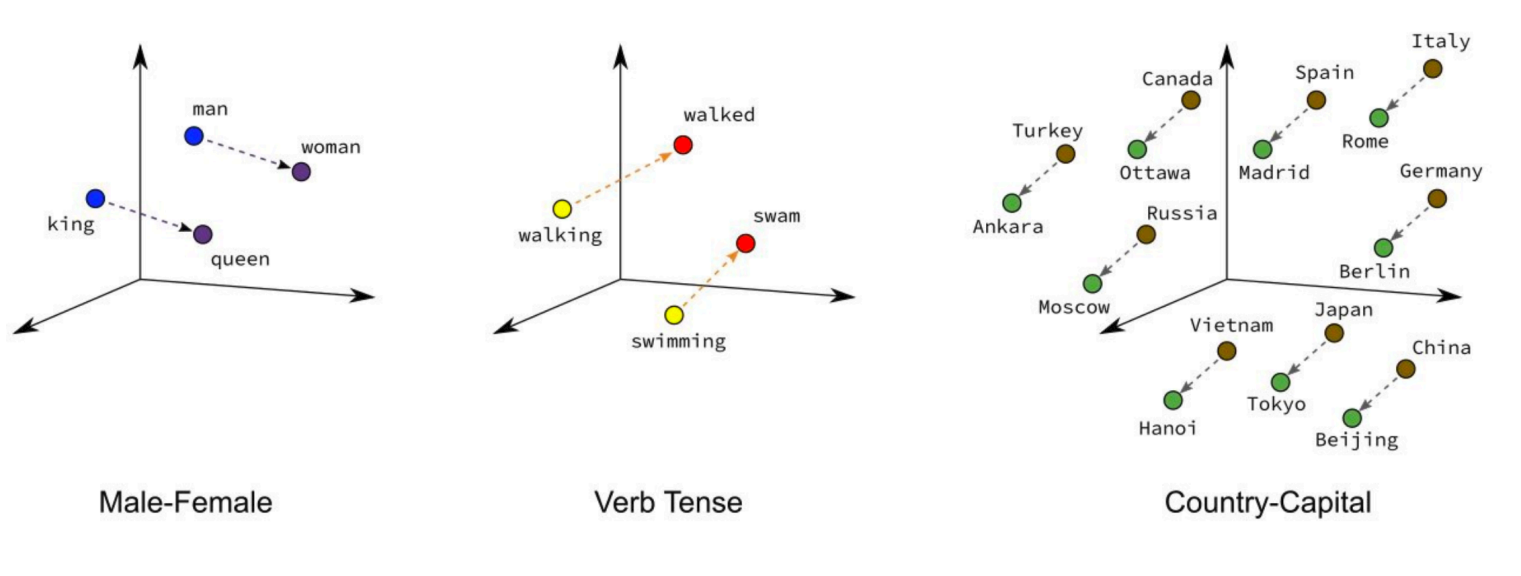
\includegraphics[scale=0.3]{screenshots/2026-05-19_1.png}
	\end{center}
	But the question that this brings up is how do we train semantics-encoding embeddings of words?
\end{parag}

\begin{parag}{Training}
    In a supervised model, the training comes down to optimizing the embeddings for a specific task (e.g., sentiment analysis). However this may or may not generalize well. And as for unsupervised we also need something in order to learn or to \important{self supervised}. The solution to this
	\begin{center}
	    Rely on the context in which words occur to learn their meaning
	\end{center}
	The context in this case is the set of words that occur nearby, to do so there is some standard approaches such as Word2Vec or GloVe.
	
\end{parag}

\begin{parag}{Individual words}
    Here what we have done so far is to find a representation for each word, however this is not the best thing to do as not all words are indicative of the category, some words are even misleading. Therefore, instead of modeling words, the standard approach consists of modeling a complete sentence or a document as a sequence. 
	\begin{subparag}{Remark}
	    Note that each individual word is still modeled as a vector as discussed previously.
	\end{subparag}
\end{parag}

\begin{parag}{Recurrent neural networks}
    The solution to model each of this block is \important{recurrent neural networks}, what this essentially is, it is a neural network with a feedback loop.
	\begin{center}
	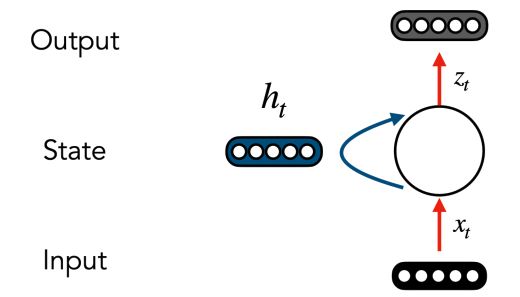
\includegraphics[scale=0.2]{screenshots/2026-05-19_2.png}
	\end{center}
	By unrolling the RNN across al time steps we get a full computation graph
	\begin{center}
	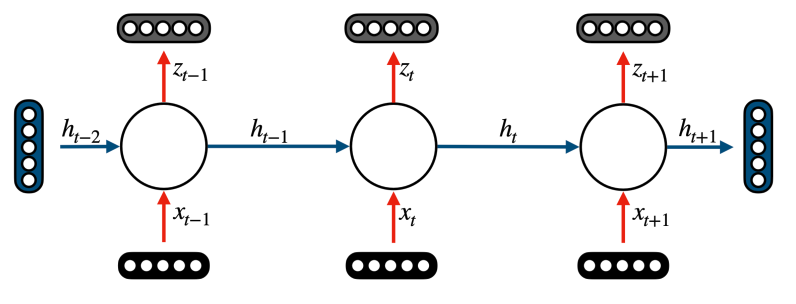
\includegraphics[scale=0.2]{screenshots/2026-05-19_3.png}
	\end{center}
	This allows learning from entire sequence history, regardless of length. Therefore what this is essentially doing is:
	     We have a hidden state $h_t$ which gets updated as each new word is processed. The update rule is typically (given by claude)
			\begin{align*} 
				h_t = f\left(W_h \cdot h_{t-1} + W_x \cdot x_t + b\right)
			\end{align*}
			Where 
			\begin{itemize}
			\item $h_{t-1}$ is the previous hidden state (the 'memory' of everything seen so far)
			\item $x_t$ is the current word vector
			\item $W_h, W_x$ are learned weight matrices
			\item $f$ is a non-linear activation 
			\end{itemize}
		The important thing to understand here is that $h_t$ acts as a \important{compressed summary of the entire sequence up to position $t$} .
\end{parag}


\begin{parag}{RNN for classification}
    Remember how did we define classification before, it what just an output projection followed by a softmax. Therefore, all we need to do here is to take our RNN model, and after the last given output, we apply our classifier. For instance if our goal was to see whether each word is a noun adverb etc...  Our model could look like this
	\begin{center}
	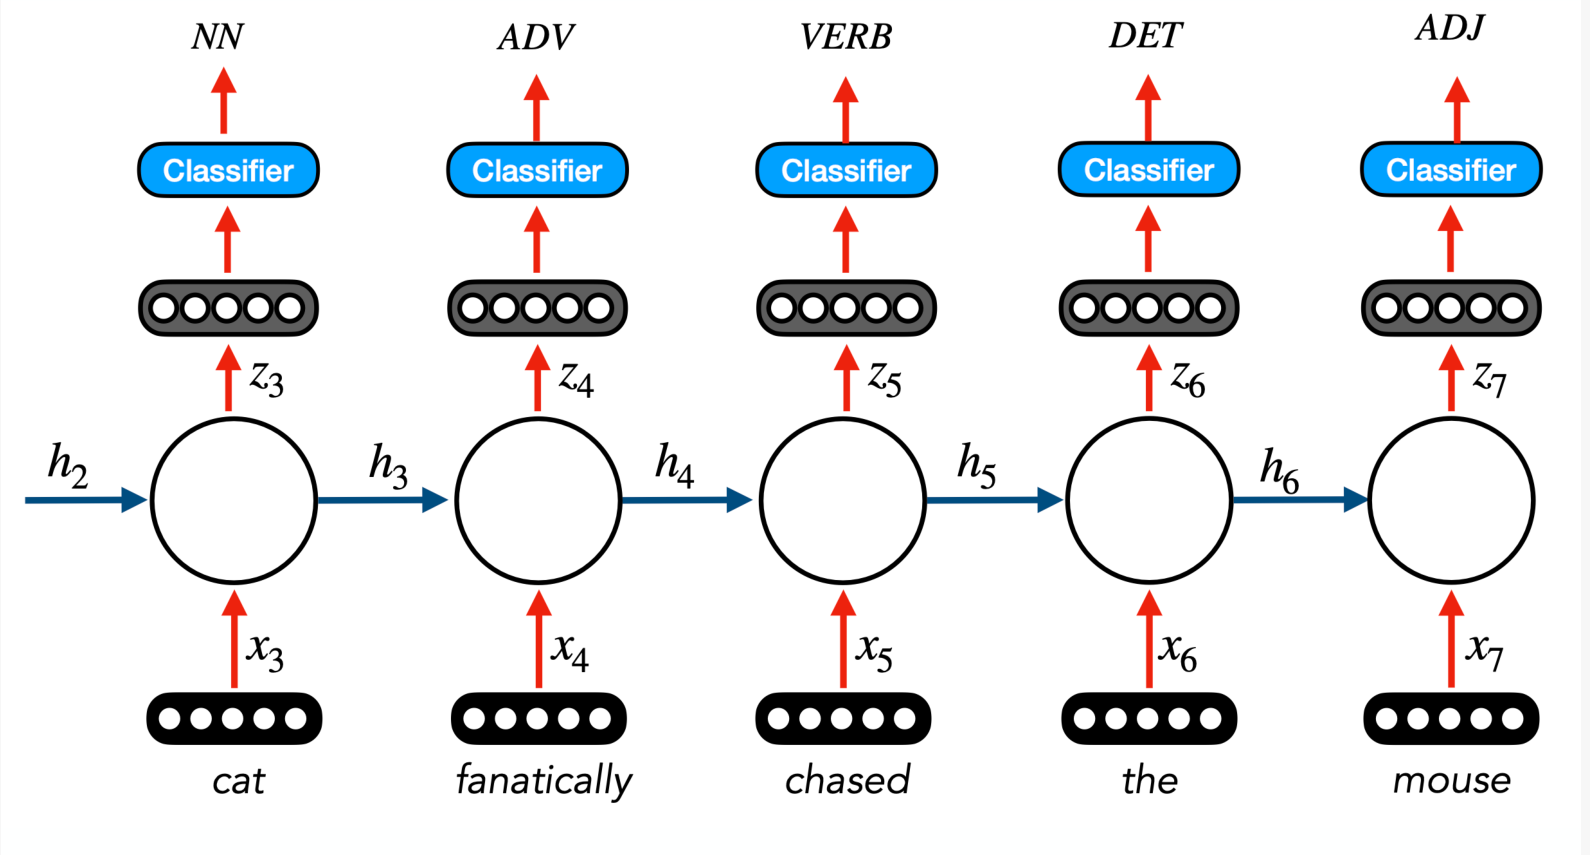
\includegraphics[scale=0.15]{screenshots/2026-05-19_4.png}
	\end{center}
	Where as if we wanted to generate text, we would output a word at each step and use is as a new word onto the next NN:
	\begin{center}
	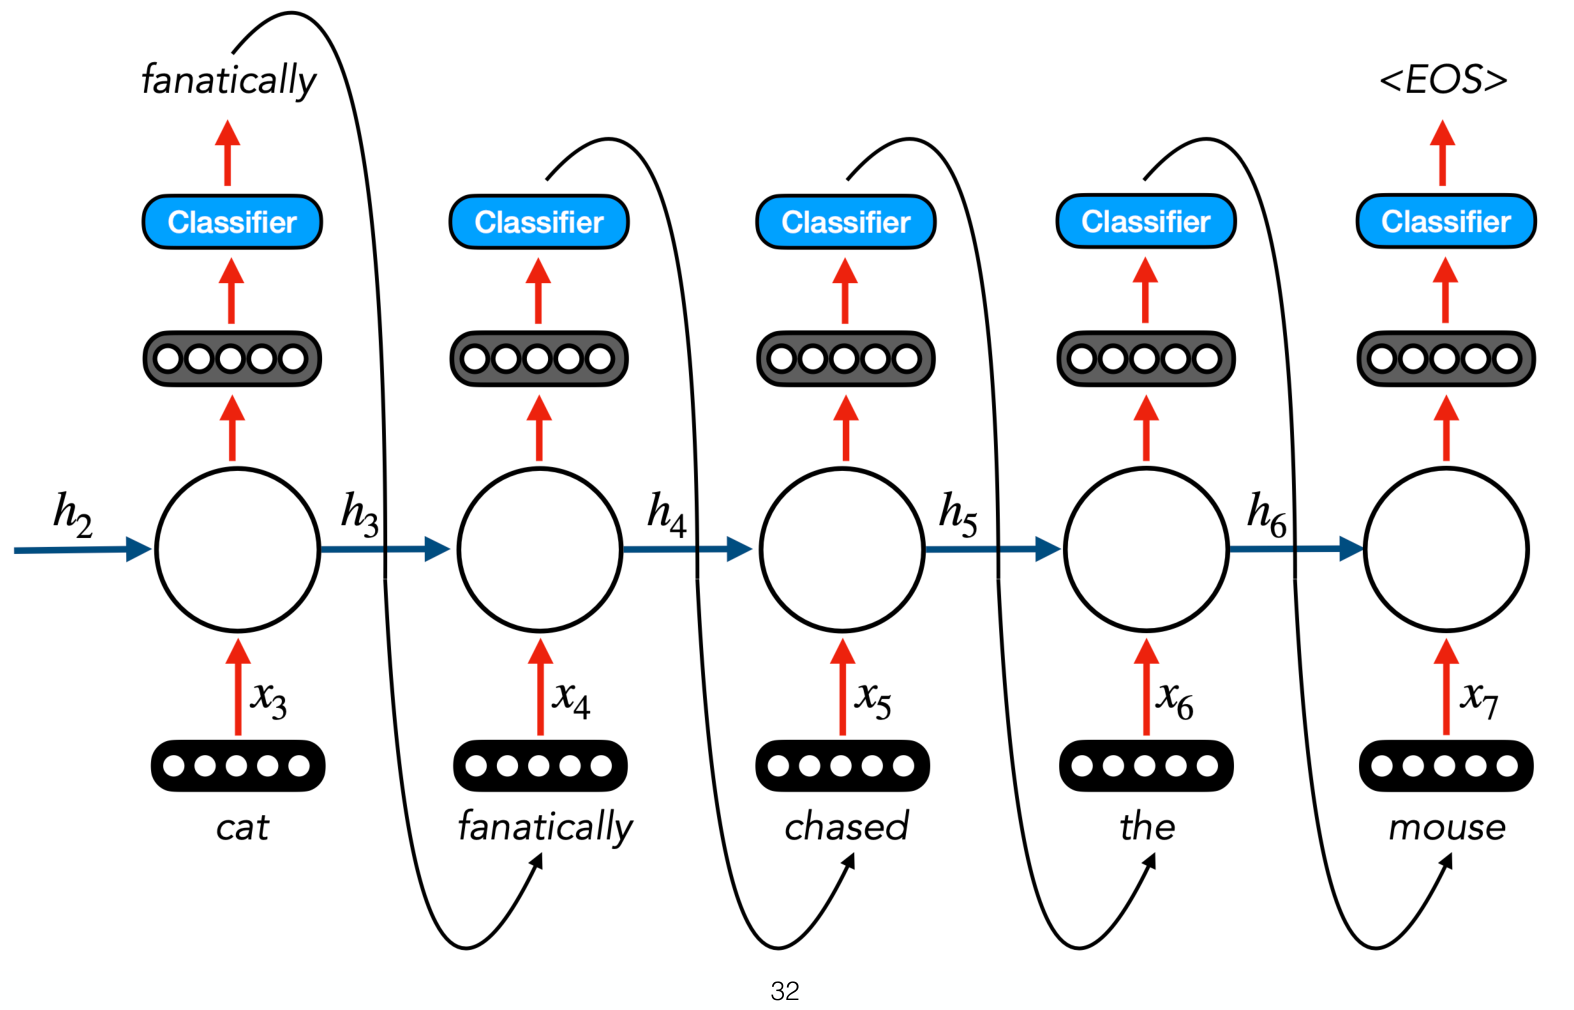
\includegraphics[scale=0.15]{screenshots/2026-05-19_5.png}
	\end{center}

\end{parag}

\begin{parag}{Different types of RNNs}
    As we have seen before (I guess claude was right), the standard RNN definition is as follow 
	\begin{align*} 
		h_t = \sigma\left(W_{hx}x_t + W_{hh}h_{t-1} + b_h\right)\\
		z_t = \sigma\left(W_{zh}h_t + b_z\right)
	\end{align*}
	we also have other types such as 
	\begin{itemize}
		\item Long Short-Term Memory (LSTM) - Hochreiter \& Schmidhuber, 1997
		\item Gated Recurent Unit (GRU) - Cho et al., 2014
	\end{itemize}
	
\end{parag}


\begin{parag}{Training an encoder-decoder model}
	Before knowing what encoder-decoder models are first, what are encoder and decoder models?
	\begin{subparag}{Encoder}
	    The encoder reads the \important{input sequence} word by word, updating its hidden state at each step. Its job is to produce a representation of the input. In the basic version, you just take the \important{final hidden state $h_T$} as a summary of the whole input sentence. (this is the classical RNN)
	\end{subparag}
	\begin{subparag}{Decoder}
	    The decoder takes that representation and \important{generates the output sequence, one word at a time} (this is the RNN for generation)
	\end{subparag}
	The flow of this model 
	\begin{align*} 
		\underbrace{x_1, x_2, \ldots, x_T}_{\text{encoder reads this}} \to \underbrace{h_T}_{\text{bottleneck}} \to \underbrace{y_1, y_2, \ldots, y_{T'}}_{\text{decoder generates this}}
	\end{align*}

    As we already know, the goal is to minimize the average cross-entropy over all tokens:
	\begin{align*} 
		\mathcal{L} =  \sum_{t= 1}^{T} - \log\left(Py_t | y_1, \ldots, y_{y-1}, x_1, \ldots, x_n\right)
	\end{align*}
	What this loss is asking is '\textit{at each step $t$, how suprised were we by the correct next token $y_t$ given everything before it?}'. So for each position $t$, the decoder outputs a probability distribution over the whole vocabulary, and you just check how much probability mass was assigned to the correct word $y_t$.
	To do so we backpropagate gradients through both the decoder and the encoder.
\end{parag}

\begin{parag}{Limitation}
    \begin{center}
		'\textit{you can't cram the meaning of a whole \%\&@#\&ing sentence into a single \$*(\&@ing vector!)}' -- Ray Mooney (NLP Prof. at UT Austin)
    \end{center}
	However turning a whole sentence into a single vector leads to a massive compression of information. This challenges to learn long-range dependencies/interactions. The reason on this is the same as we have already talked about previous section, when dealing with long series of network (meaning gradients of gradients of gradients... Often the first time steps (the first words) get exponentially converging to $0$, this implies that early words are '\textit{forgotten}'), LSTMs were the first major attempts to address this. We introduce a cell state $c_t$ (a separate memory track) alongside the hidden state $h_t$, controlled by three gates:
	\begin{itemize}
	    \item Forget gate $f_t$: how much of the previous cell state to erase
	    \item Input gate $i_t$: how much of the new input to write into memory
	    \item Output fate $o_t$: how much of the cell state to expose as $h_t$
	\end{itemize}
	Each gate here is a sigmoid, acting like a soft on/off switch. This lets the netwrosk selectively remember or forget over long sequences, which helps but doesn't fully solve the compression problem.
\end{parag}

\begin{parag}{Incorporating attention}
	As seen before at each encoder time step, there is an output of the RNN. The idea here is to use the output of the decoder LSTM to compute an \important{attention} (i.e., mixture) over all the $_{t}^{e}$ outputs of the encoder LSTM. 
	\begin{subparag}{Intuition}
	    Instead of forcing everything into a single final vector $h_T$, \important{attention} keeps \important{all} the hidden state $h_1, \ldots, h_T$ and at each step computes a weighted mixture 
		\begin{align*} 
			c_t = \sum_{i} \alpha_{it} \cdot  h_i
		\end{align*}
		Where each $a_{ti}$ are learned weights representing '\textit{how relevant is word $i$ for the current step?}'. This way the model can directly reach back to any earlier state rather than relying on it surviving compression.
	\end{subparag}
	\begin{center}
	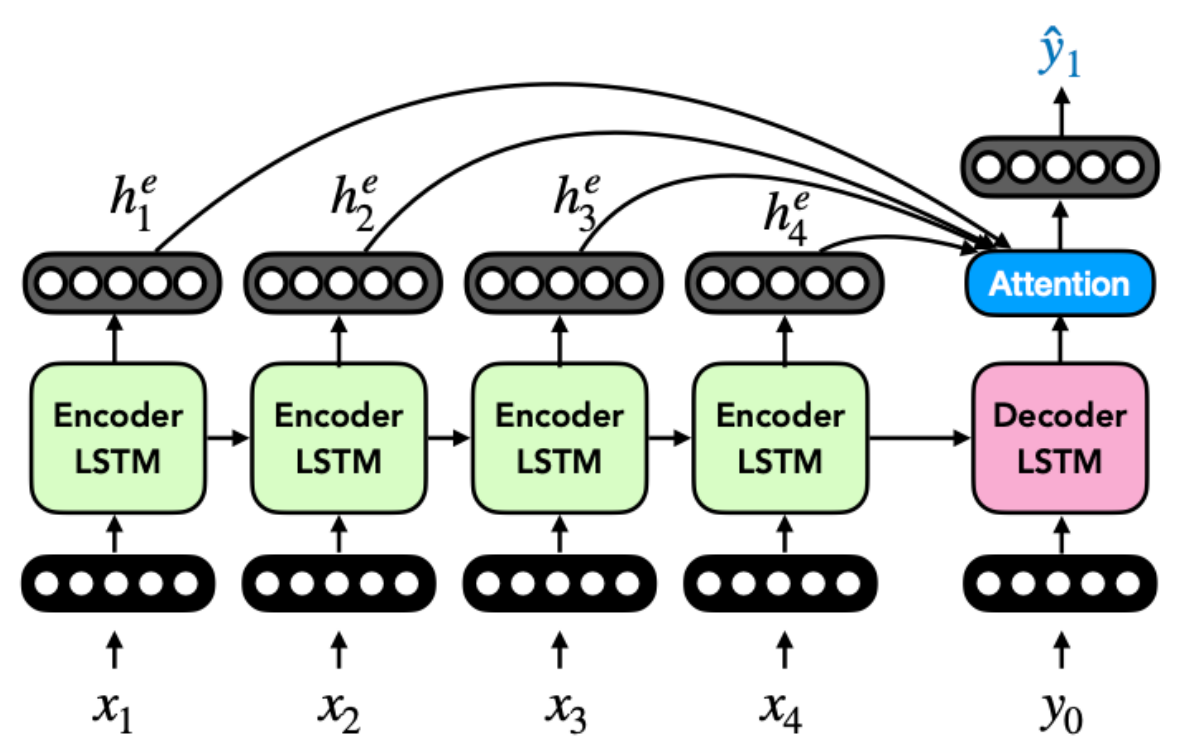
\includegraphics[scale=0.15]{screenshots/2026-05-19_6.png}
	\end{center}
\end{parag}


\begin{parag}{Attention function}
    The goal of this function is to compute pairwise similarity between each encoder hidden state and decoder hidden state ('idea of what to decode'). We define 
	\begin{align*} 
		h_{t}^{e} =  \text{encoder output hidden states}\\
		h_{t}^{d} = \text{decoder output hidden state}
	\end{align*}
	\begin{subparag}{Note}
	    We also call $h_{t}^{e}$ the keys and $h_{t}^{d}$ the query
	\end{subparag}
	Therefore we define 
	\begin{align*} 
		a_1 =  f\left(h_{1}^{e}, h_{1}^{d}\right), \mathspace a_2 = f\left(h_2^{e}, h_{1}^{d}\right)
	\end{align*}
	Here we are asking '\textit{how relevant is encoder position $i$ for what I'm currently trying to decode?}'.
	As you could have guessed there is a lot of attention function $f$ out there here are three:
	\begin{subparag}{Multiplicative}
	    \begin{align*} 
			a =  h^{e}Wh^{d}
		\end{align*}
	\end{subparag}
	\begin{subparag}{Linear}
	    \begin{align*} a = v^{T}\phi\left(W\left[h^{e};h^{d}\right]\right) \end{align*}
	\end{subparag}
	\begin{subparag}{Scaled dot product}
	    \begin{align*} a = \frac{\left(Wh^{e}\right)^{T}\left(Uh^{d}\right)}{\sqrt{d}} \end{align*}
	\end{subparag}
	This convert the pairwise similarity scores to a probability distribution (using softmax) over encoder hidden states and compute weighted average. This mean that we have all $a_i$ define as 
	\begin{align*} 
		a_i = f\left(h_{i}^{e}, h_{1}^{d}\right)
	\end{align*}
	then we normalize those scores into a proper distribution 
	\begin{align*} 
		\alpha_t = \frac{e^{a_t}}{\sum_{j} e^{a_j}}
	\end{align*}
	Therefore $a_i \in \left[0, 1\right]$ and they sum to $1$. We can then compute the weighted average 
	\begin{align*} 
		\widetilde{h}_{1}^{d} =  \sum_{t= 1}^{T}\alpha_t h_{t}^{e}
	\end{align*}
	This is the mixture that we talked about before.
	\begin{center}
	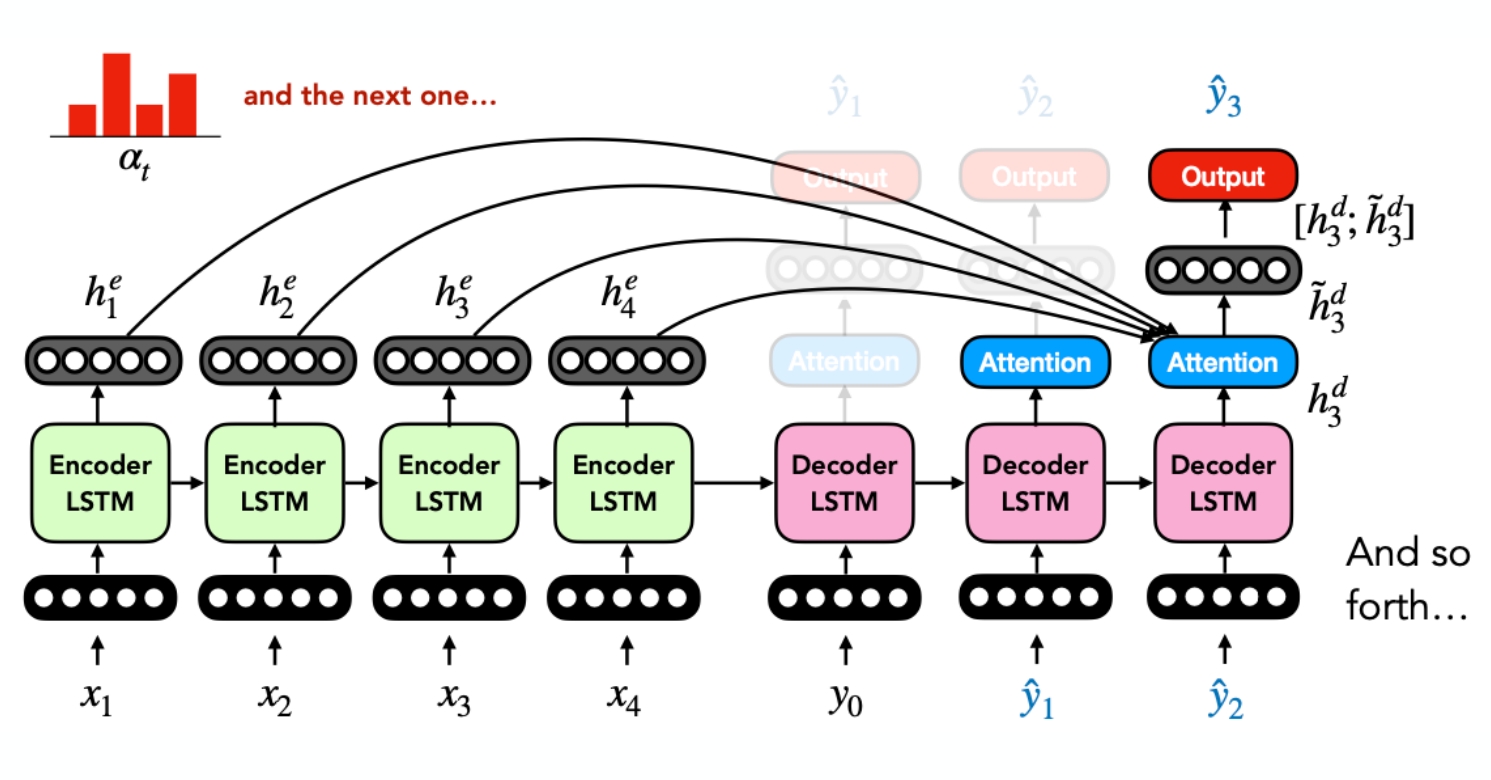
\includegraphics[scale=0.15]{screenshots/2026-05-19_8.png}
	\end{center}
\end{parag}
\begin{parag}{Interpretability?}
    As said before attention can be visualised based on the score given to each encoder hidden state. But what is focused on when each word is generated? Training with attention gives us implicit alignment for free! Our weights $a_t$ form a matrix which mean that we can therefore plot as a heatmap where $\alpha_{ti}$ tells us how much decoder step $t$ attends to encoder position $i$.
	\begin{center}
	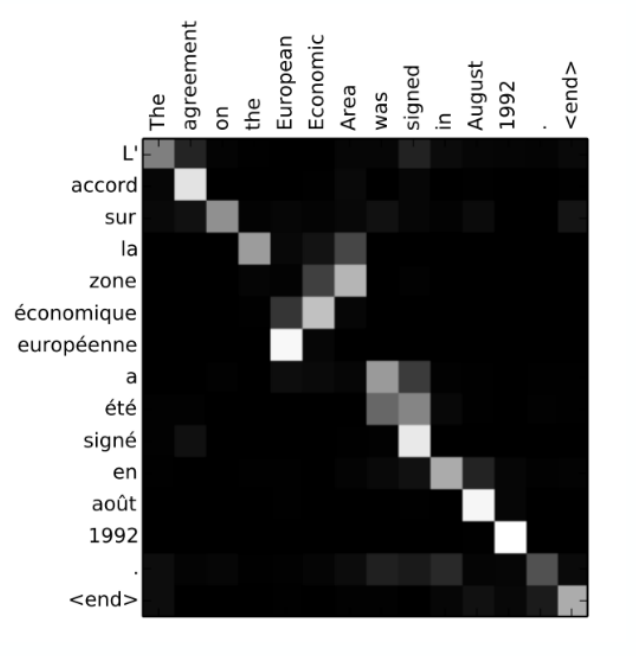
\includegraphics[scale=0.2]{screenshots/2026-05-19_9.png}
	\end{center}
	So here when we are trying to translate English \textrightarrow French, we would typically see a near diagonal pattern for words that translate in similar order. Off-diagonal jumps for reorderings.  
\end{parag}

\begin{parag}{Problem: Encoder is recurrent}
    There is a big performance issue here, recurrent function can't be parallelized because previous state needs to be computed to encode next one. Encoder hidden states must still be computed in series. The solution to this are transformers.
\end{parag}


\subsection{Transformer}
Transformers are made up of encoder and decoder, where both encoder and decoder are made up of multiple cascaded transformers blocks. (there is a slightly different architecture in encoder and decoder transformer blocks). Blocks are generally made up of \important{multi-headed attention} layers (self attention) and \important{feedfoward} layers. What this implies is that we don't have recurrent computations anymore. Multiple cascaded blocks are important here, they are analogous to how deep CNNs learn. Early block might learn syntatic relationship whereas deeper block learn more semantic/abstract ones.
\begin{parag}{Transformers vs RNNs}
    RNNs process sequence step by step, word 1, then word 2, then word 3. The only way word 1 can influence word 5 is by surviving through the hidden state chain. Transformers \important{abandon recurrence entirely} and instead let every word talk to every other word simultaneously. More concretely let us take a transformer block. Instead of a hidden state that gets updated, a transformer block takes a \important{whole sequence of vectors} and outputs a \important{whole sequence of vectors}
	\begin{align*}
		\left[x_1, \ldots, x_T\right] \overset{\text{transformer block}}&{\xrightarrow{\hspace*{3cm}}} \left[z_1, \ldots, z_T\right]
	\end{align*}
	Each output $z_i$ is an enriched representation of word $i$, informed by all other words via self-attention.
\end{parag}

\begin{center}
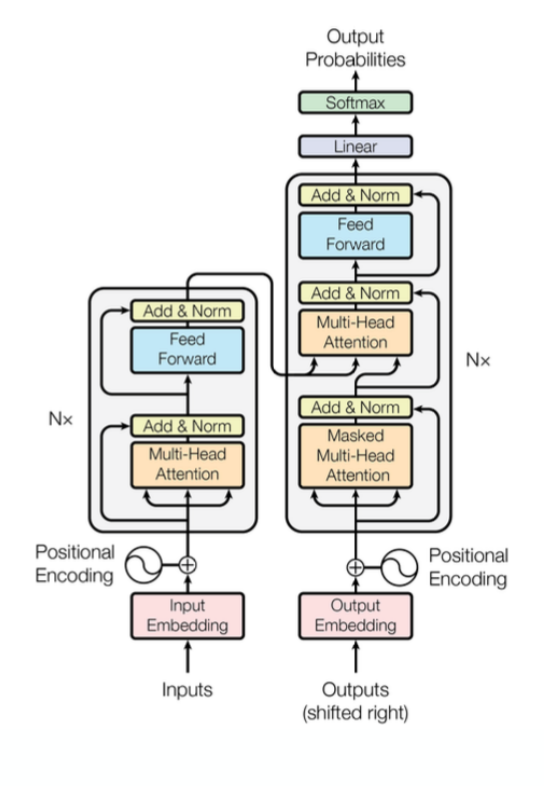
\includegraphics[scale=0.2]{screenshots/2026-05-19_10.png}
\end{center}


\begin{parag}{Self-attention}
    In the RNN attention we saw earlier, attention as between two different sequences, the encoder states and the decoder states. \important{Self-attention} is attention where the sequence attends to itself, every position looks at every other position in the \important{same} sequence to build a better representation.
	\begin{subparag}{How it works}
	    For each position $i$ in the sequence, you create three vector from the word embedding 
		\begin{itemize}
		\item Query $q_i$: what am I looking for?
		\item Key $k_{j}$: what do I contain?
		\item Value $v_j$: what do I actually pass along?
		\end{itemize}
		Then the attention score between position $i$ and $j$ is 
		\begin{align*} 
			a_{ij} = \frac{q_i \cdot k_j}{\sqrt{d_k}}
		\end{align*}
	\end{subparag}
	\begin{center}
	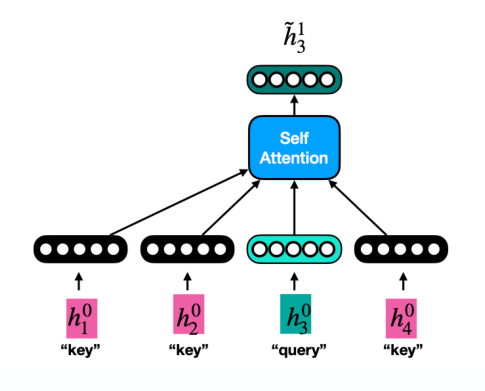
\includegraphics[scale=0.4]{screenshots/2026-05-19_12.png}
	\end{center}
	We have that for each attention computation, every element is a key and value, and one element is a query.The $Q, K, V$ vectors are obtained by learned linear projections 
	\begin{align*} 
		q = W^{Q}h_{s}^{e} \mathspace K =  W^{K}\left\{h_{t}^{e}\right\} \mathspace V = W^{V}\left\{h_{t}^{e}\right\}
	\end{align*}
	Then we do this computation for each $\widetilde{h}_{i}^{1}$
	\begin{center}
	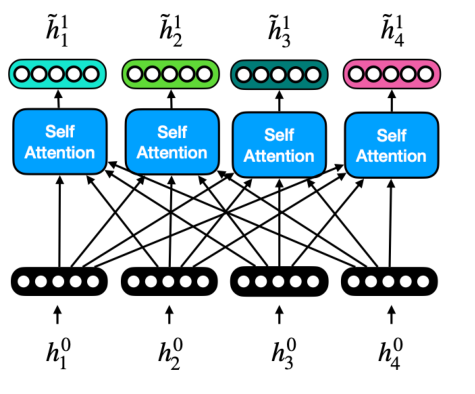
\includegraphics[scale=0.3]{screenshots/2026-05-19_13.png}
	\end{center}
	Where each $\widetilde{h}_{i}^{1} =  \text{Attention}\left(h_{i}^{0}, \left\{h_{t}^{0}\right\}_{t= 0}^{t= 3}\right)$\\
	$ $\\
	Therefore the full computation is defined as 
	\begin{align*} 
		a = \frac{\left(W^{Q}q\right)\left(W^{K}K\right)}{\sqrt{d}} \overset{\text{softmax}}&{\xrightarrow{\hspace*{2cm}}} \alpha \overset{\text{weighted sum}}&{\xrightarrow{\hspace*{2cm}}} \widetilde{h}^{e} =  W^{O}\alpha\left(VW^{V}\right)
	\end{align*}

\end{parag}

\begin{parag}{Example}
    Let us now take the diagram below to understand the whole picture. 
	\begin{center}
	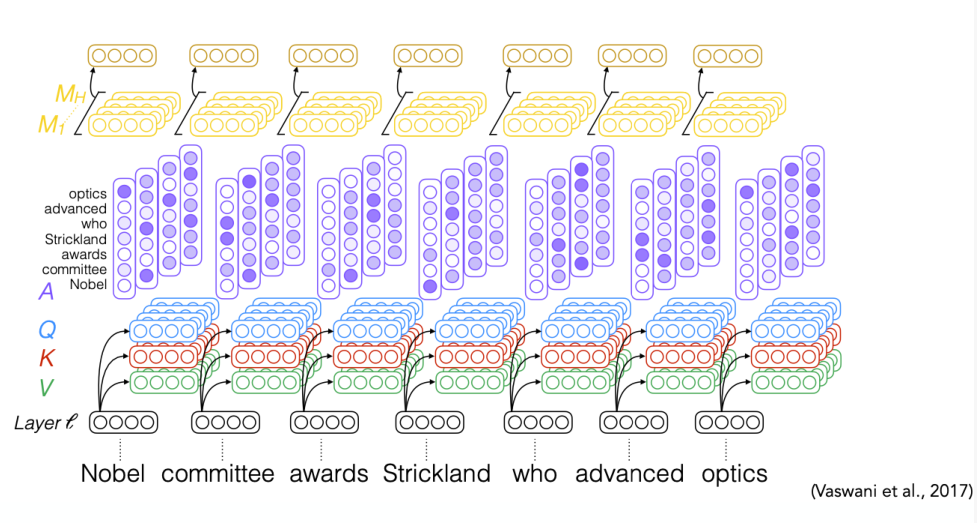
\includegraphics[scale=0.3]{screenshots/2026-05-19_14.png}
	\end{center}
	\begin{subparag}{Bottom layer $l$}
	    The small white boxes at the bottom are the current hidden state $h_{i}^{l}$ for each word, this is the input to this transformer block.
	\end{subparag}
	\begin{subparag}{$Q, K, V$ projections}
	    For \important{every word simultaneously}, you compute the three projections:
		\begin{itemize}
		    \item $Q$ (blue): queries
		    \item $K$ (red): keys
		    \item $V$ (green): values
		\end{itemize}
		The arrow show that every word connects to every other word. This is a pairwise self-attention computation.
	\end{subparag}
	\begin{subparag}{Attention outputs}
	    This is the thing in purple vectors, those are the outputs after computing $\alpha$ and the weighted sum of values. Notice that \important{varying shading} in the purple vectors means higher activation, showing how different word contributed to the current output.
	\end{subparag}
	\begin{subparag}{Multi-head $M_1, \ldots, M_H$}
	    This is the main idea, instead of computing attention \important{once}, we do it $H$ times in parallel, each with different $W^{Q}, W^{K}, W^{V}$ matrices. Each head can learn to attend to \important{different types of relationship} (syntactic, coreference, ...). Then the output of all heads are then \important{concatenated} and \important{projected} back to the original dimension.
	\end{subparag}
	But why do we even need multi-head? A single attention head produces one weighted mixture, it's forced to compress all relationship into one distribution. Multiple heads let the model capture \important{several different relationship types simultaneously}, which is much more expressive.
\end{parag}













\begin{parag}{Transformer block}
    The Multi-headed attention is the main innovation of the transformer model 
	\begin{center}
	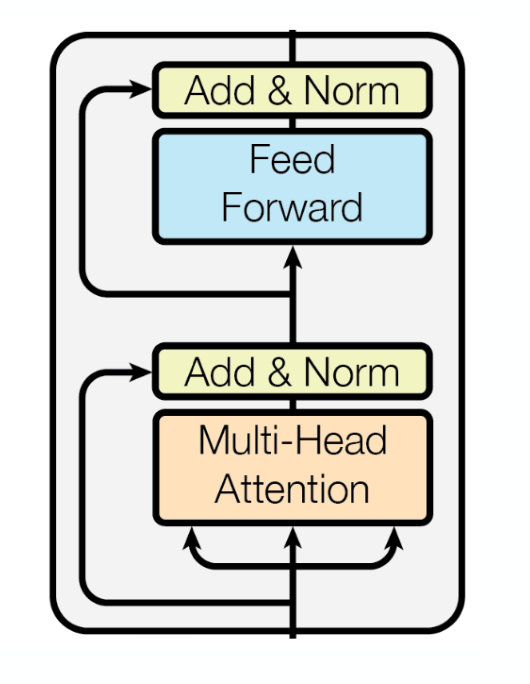
\includegraphics[scale=0.3]{screenshots/2026-05-19_15.png}
	\end{center}
	Each block here is also composed of:
	\begin{itemize}
	    \item A layer of normalizations
	    \item A feedfoward network
	    \item residual connections
	\end{itemize}
\end{parag}
\begin{parag}{Full transformer}
    In order to have a full transformer encoder, all we need to do is to put multiple cascaded transformer block together which we'll \important{build up} compositional representation of inputs.\\
	$ $\\
	On the other hand, when looking for the decoder (right) this is similar to encoder where:
	\begin{itemize}
	\item First layer of block is \important{masked} multi-headed attention
	\item Second layer is multi-headed attention over final layer encoder outputs (\important{cross attention})
	\item Third layer is feed-forward network
	\end{itemize}
	\begin{center}
	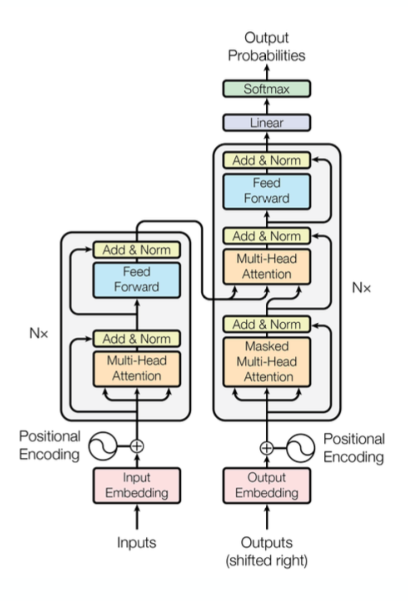
\includegraphics[scale=0.3]{screenshots/2026-05-19_16.png}
	\end{center}
	
\end{parag}


\begin{parag}{Masked multi-head self attention}
    As we have seen, self-attention can attend to any token in the sequence. However for the decoder, we don't want tokens to attend to future tokens, if the decoder is used to generate text (i.e., machine translation). As during training we have full target sequence, this is different here right. During generation, we can only use words we have already produced. The constraint is: when predicting a word $t$, we should only be allowed to look at words $1, \ldots, t-1$ and \important{never} $t + 1, t+2, \ldots$
	\begin{subparag}{Concrete example}
		Say the target is '\textit{Novel committee awards Strickland}'. When predicting 'awards':
		\begin{itemize}
		    \item We can attend to 'nobel' and 'committee'
		    \item We \important{cannot} attend to 'Strickland', it hasn't been generated yet
		\end{itemize}
		If the model could peek at future words during training, it would just cheat, learning nothing useful, since at test time,those future word don't exist yet.
	\end{subparag}
	How masking works is pretty simple, we simply set the attention scores for future position to $-\infty$ before the softmax function:
	\begin{align*} 
		a_{ij} = \begin{cases}
			\frac{q_i k_j}{\sqrt{d}} \mathspace \text{ if } j \leq i\\
			-\infty \mathspace \text{ if } j > i
		\end{cases} 
	\end{align*}
	Which implies when we apply to softmax 
	\begin{align*} 
		\alpha_{st} = \frac{e^{a_{st}}}{\sum_{j}e^{a_{sj}}} = 0
	\end{align*}
	when $s < t$. Therefore, our attention matrix is a lower triangle matrices.
\end{parag}


\begin{framedremark}
A question I asked claude which was (after the 100th ones) when we are training, we are essentially training models of models, also if we don't know the length of the sentence, how do we train a model here without knowing its size?\\
$ $\\
\textbf{Answer}
You're training one single model — not a model of models. The encoder and decoder are just two components of the same network sharing a training objective. The loss is still the same cross-entropy:
\begin{align*} 
	\mathcal{L} = \sum_{t= 1}^{T} - \log P\left(y_t | y_1, \ldots, y_{t - 1}, x_1, \ldots, x_n\right)
\end{align*}
You have paired examples (input sentence, target sentence), and you backpropagate gradients through both decoder and encoder simultaneously. Everything is just one big computation graph with shared weights being updated together.\\
$ $\\
\textbf{Variable length sequences}
We have already kind of see it in RNN but here the issue is that we need to train our model before knowing the size of the input. To do so when we have to short sentence in comparisons to the model input size we add padding using special token (e.g. $\left[PAD\right]$) make those positions ignored (set to $-\infty$ before the softmax). We can also put special token such as $\left[EOS\right]$ at the end of the sentence (we have seen one in the previous diagram) in order to have a model that can even itself choose when to end its generation. Okay this is nice but what is the concrete difference between me sending a 10 words sentence to claude or a 10000 words sentence to claude?\\
$ $\\
As transformer have a fixed maximum sequence length, which is called the \important{context window}. Therefore when having a 10 word sentence, it get padded up to the max length, whereas if we have a sentence longer than the context window: it gets \important{truncated}, we simply lose the rest. The model never sees it. (this is the reason on why some model hallucinated or just repeat themself after long discussion, the context window is full). 
\end{framedremark}



\begin{parag}{Cross attention}
    \important{Cross attention} is the same as classical attention as in the RNN encoder-decoder. The difference here is that the attention function is the output of the masked multi-headed attention in the decoder (e.g., a decoder state). The keys and values are the output of the \important{final} encoder transformer. Once again, a representation from the decoder is used to \important{attend} to the encoder outputs.
	\begin{center}
	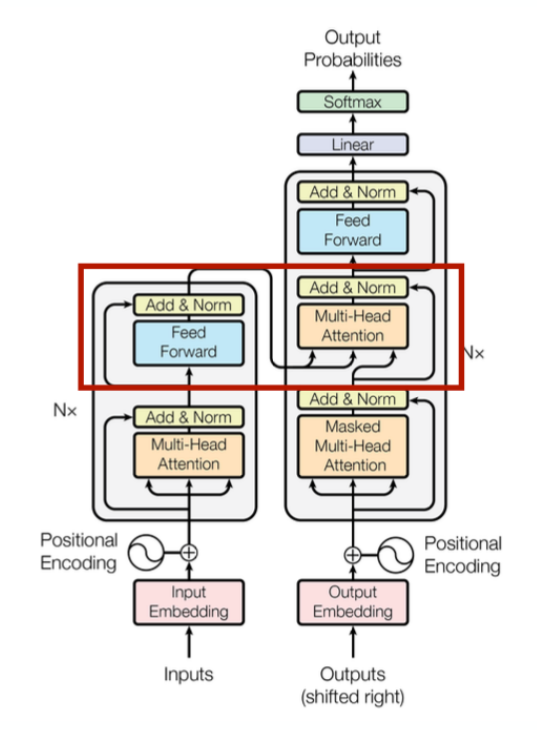
\includegraphics[scale=0.2]{screenshots/2026-05-20.png}
	\end{center}
	To resume this a bit better, the difference with self-attention is 
	\begin{itemize}
	    \item The \important{Query} $Q $ \textrightarrow comes from the \important{decoder} (masked self-attention output) and asks 'what am I trying to generate?'
	    \item The \important{Key} $K$ and \important{Value} $V $ \textrightarrow comes from the \important{final encoder layer} and asks the question "what was in the input?"
	\end{itemize}
	So unlike self-attention where everything came from the same sequence, cross attention \important{mixes two difference sequences}
	\begin{align*} 
		\underbrace{\text{decoder state}}_{\text{Query}} \to \text{cross attention} \leftarrow \underbrace{\text{final encoder output}}_{\text{Keys \& Values}}
	\end{align*}
	At each decoder step, the decoder asks: "\textit{given what I want to generate, which part of the input sentence should I focus on?}"\\
	$ $\\
	Now the question on why we only "\textit{care}" about the last final layer even though we have already computed all previous one is that the final encoder layer contains the \important{most enriched representations}, each token has already been 

\end{parag}


\begin{parag}{Position Embeddings}
	The issue we have with what as been said before about context attention etc. is that for instance, shuffling tokens doesn't change the result of the attention. This is not really what we want right? For instance the sentence '\textit{I eat apple and not pear because I hate it}' and the sentence '\textit{I eat pear and not apple because I hate it}' we'll give us the same output. Therefore for each token, it would be useful to add to it information about the \important{position}, to embeds positions (idk if that's a saying). To do so we will use a sinusoid function that is offset by a phase shift proportional to the sequence position. The positional encoding for the index $i$ would be given as 
	\begin{align*} 
		p_i = \begin{pmatrix} \sin\left(\frac{1}{10000^{2 \cdot  \frac{1}{d}}}\right) \\ \cos\left(\frac{i}{10000^{2 \cdot \frac{1}{d}}}\right)\\ \vdots \\ \sin\left(\frac{i}{10000^{2 \cdot  \frac{d}{2d}}}\right) \\  \cos\left(\frac{i}{10000^{2 \cdot  \frac{d}{2d}}}\right)\end{pmatrix} 
	\end{align*}

\end{parag}



\paragraph{GPT: Generative Pretrained Transformer}%
\label{par:GPT: Generative Pretrained Transformer}
Here we have two words giving hints about what this model should do, it is \important{generative}, meaning it generates texts and it is \important{pretrained} meaning it has been trained on a lot of data. Those are also called as a decoder transformer. However the actual GPT block mixes design of encoder and decoder from the original transformer. It also uses masked multi-headed self-attention (on the decoder) meaning it cannot see the future. We also have no cross attention; we only compute a self-attention over its history in each block (encoder).

\begin{parag}{Training}
    GPT are trained on an enormous amount of data, on the TorontoBooks corpus (7000 unpublished books ($\sim$ 13 GB)). Each corpus is segmented into windows of 512 tokens. The training is done by trying to predict the next word.
\end{parag}
\begin{parag}{Fine tuning}
    After pre-training, model can be fine-tuned by training on individual datasets. Pretrained model are used as initialisation for training on individual tasks.
	\begin{center}
	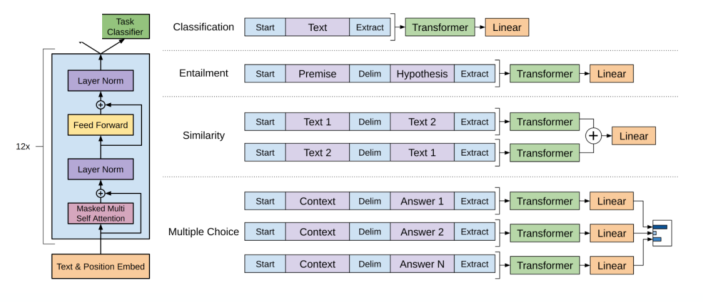
\includegraphics[scale=0.3]{screenshots/2026-05-22.png}
	\end{center}
\end{parag}







\paragraph{Transformers for images}%
\label{par:Transformers for images}
When trying to use transformers for images, the simplest way is to consider the pixels as words 
\begin{center}
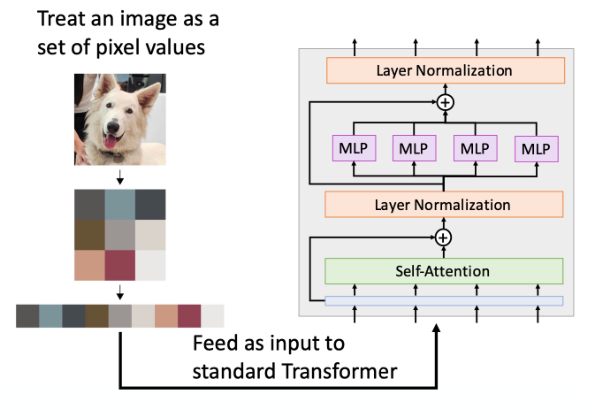
\includegraphics[scale=0.3]{screenshots/2026-05-22_1.png}
\end{center}
But this is just an enormous  amount of data, so instead let us try to use patches of images.
\begin{center}
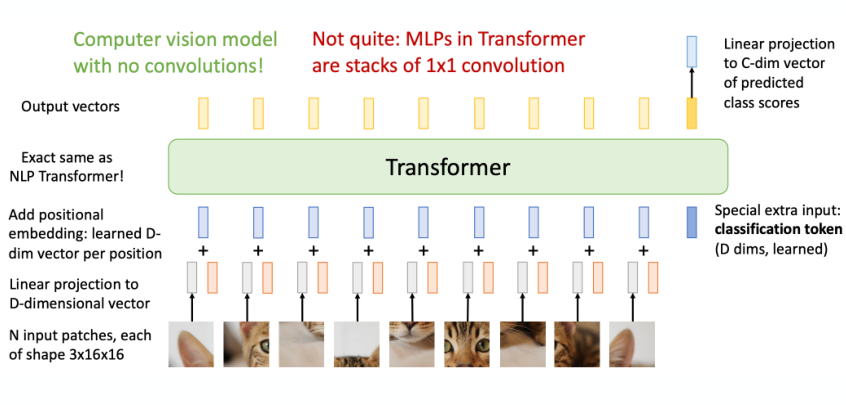
\includegraphics[scale=0.3]{screenshots/2026-05-22_2.png}
\end{center}

